% ============================================================
%  LIVRABLE COMPLET — Time'Eats — Cellule PMO
%  Partie I  : Gestion du portefeuille (méthodologie, référentiel, cockpit)
%  Partie II : Application au projet Refonte Web
%  CESI MAALSI Semestre 2 — 2026
% ============================================================
\documentclass[11pt,a4paper,oneside]{report}

\PassOptionsToPackage{backend=bibtex}{biblatex}
\usepackage{style/consulting}
\usepackage{graphicx}
\graphicspath{{img/}{.}}
\addbibresource{references.bib}

\hypersetup{
  pdftitle={Time'Eats — Supervision du portefeuille \& projet Refonte Web},
  pdfauthor={Cellule PMO — CESI MAALSI},
}

\pagestyle{fancy}
\fancyhf{}
\renewcommand{\headrulewidth}{0pt}
\fancyhead[L]{%
  \begin{tikzpicture}[remember picture, overlay]
    \draw[cnNavy, line width=0.5pt] (0,-0.42cm) -- (\textwidth,-0.42cm);
  \end{tikzpicture}%
  \vspace{2pt}\timeeatslogo\hspace{4pt}\small\textcolor{cnSlate}{Time'Eats \textbf{·} PMO --- Portefeuille \& Refonte Web}%
}
\fancyhead[R]{}
\fancyfoot[C]{\tiny\textcolor{cnSlate}{Document confidentiel --- Cellule PMO --- CESI MAALSI 2026}}
\fancyfoot[R]{\small\textcolor{cnSlate}{\thepage}}

% Commandes RAG
\newcommand{\ragV}{\cellcolor{cnGreen!20}\textbf{\textcolor{cnGreen}{Vert}}}
\newcommand{\ragA}{\cellcolor{cnOrange!20}\textbf{\textcolor{cnOrange}{Ambre}}}
\newcommand{\ragR}{\cellcolor{cnRed!20}\textbf{\textcolor{cnRed}{Rouge}}}

\begin{document}
\small

% ── Page de garde ────────────────────────────────────────────
\begin{titlepage}
  \pagecolor{cnNavy}
  \color{white}
  \vspace*{2.5cm}
  \begin{center}
    {\Huge\bfseries Time'Eats}\\[0.5cm]
    {\normalsize\textcolor{cnSlate} Cellule PMO --- Direction des Systèmes d'Information}\\[2cm]
    \textcolor{cnOrange}{\rule{12cm}{1.5pt}}\\[1cm]
    {\LARGE\bfseries Supervision du portefeuille de projets IT}\\[0.4cm]
    {\Large\bfseries\&}\\[0.4cm]
    {\LARGE\bfseries Pilotage du projet Refonte Web}\\[0.8cm]
    {\large Professionnalisation de la cellule PMO}\\[1cm]
    \textcolor{cnOrange}{\rule{12cm}{1.5pt}}\\[2cm]
    {\normalsize Projet Collaboratif --- CESI MAALSI --- Semestre 2}\\[0.4cm]
    {\normalsize Mai 2026}
  \end{center}
  \vfill
  \begin{center}
    \small\textcolor{cnSlate}{Portefeuille : 11 projets --- 1\,700~K€ --- DSI : 21 personnes \quad|\quad Projet Refonte Web : 300~K€ --- 6 mois}
  \end{center}
\end{titlepage}
\nopagecolor

\tableofcontents
\newpage

% ── Introduction ─────────────────────────────────────────────
\chapter*{Introduction}
\addcontentsline{toc}{chapter}{Introduction}

\textbf{Pourquoi ce document ?} Time'Eats, spécialiste de la vente et livraison de repas préparés (siège à Rennes), engage en 2026 un programme de transformation digitale. Sa DSI (\textbf{21 personnes}, \textbf{11 projets} simultanés, \textbf{1\,700~K€} de budget annuel, fort recours aux ESN) opère aujourd'hui sans cadre méthodologique partagé : chaque chef de projet (CP) applique ses propres pratiques, ses propres modèles de documents et ses propres indicateurs. La conséquence directe est l'\textbf{impossibilité de consolider le portefeuille} : la direction ne dispose ni d'une vision unifiée des avancements, ni d'un suivi budgétaire cohérent, ni d'une lecture des risques transverses.

\textbf{Ce document est le référentiel de gestion de projet} que la \textbf{cellule PMO} publie pour répondre à ce manque. Il n'est pas un livrable académique : il est le \textit{document de référence interne} que tout CP de la DSI Time'Eats doit appliquer pour cadrer, exécuter, piloter et clôturer un projet.

\begin{finding}
\textbf{Place de la cellule PMO dans l'organisation.} La cellule PMO est \textbf{transverse} à la DSI. Elle est \textbf{garante de la méthodologie}, du référentiel documentaire et du reporting consolidé. Elle \textbf{ne pilote pas les projets} (cette responsabilité reste au CP) : elle \textbf{outille les CP} (templates, indicateurs, cockpit) et \textbf{consolide pour la direction} (vue portefeuille, météo des projets, agrégats budgétaires).
\end{finding}

\textbf{Destinataires du document :}
\begin{itemize}
  \item \textbf{Primaire} --- les chefs de projet de la DSI (5 CP) : ils appliquent la méthodologie, instancient les templates et alimentent les indicateurs projet.
  \item \textbf{Secondaire} --- la DSI et la direction générale : elles consomment la vue portefeuille consolidée par le PMO.
  \item \textbf{Tertiaire} --- les ESN partenaires (Sopra Steria, Capgemini, etc.) : elles s'alignent sur les standards documentaires et les jalons de pilotage exigés par le PMO.
\end{itemize}

\textbf{Trois objectifs structurent ce référentiel :}
\begin{enumerate}
  \item \textbf{Professionnaliser la gestion de projet} via une méthodologie hybride explicite (PMBOK 7\textsuperscript{e} édition + Scrum), organisée en 4 piliers (gouvernance, exécution bimodale, capacitaire \& ESN, standardisation du suivi) --- Ch.\ 2.
  \item \textbf{Uniformiser les documents} internes et externes via un \textbf{référentiel de 26 templates LaTeX versionnés}, couvrant les 5 phases PMBOK et applicables à tous les projets du portefeuille --- Ch.\ 3.
  \item \textbf{Alimenter une plateforme live de KPI} : chaque indicateur projet remonte automatiquement vers le \textbf{Cockpit DSI}, consultable en temps réel par les CP (vue micro) et la direction (vue macro) --- Ch.\ 3 et 4.
\end{enumerate}

\textbf{Ce livrable est structuré en deux parties complémentaires :}

\begin{itemize}
  \item \textbf{Partie I --- Gestion du portefeuille} (Ch.\ 1--4). Présente la \emph{méthodologie partagée par tous les projets} : enjeux et gouvernance du portefeuille, méthodologie hybride à 4 piliers, référentiel documentaire commun (26 templates LaTeX avec chemins), référentiel d'indicateurs en cascade, et tableau de bord de supervision (Cockpit DSI).
  \item \textbf{Partie II --- Application au projet Refonte Web} (Ch.\ 5--7). Démontre l'\emph{instanciation concrète} de la méthodologie sur un projet du portefeuille (Refonte Web --- 300~K€ --- ESN Sopra Steria --- Go-Live 30/09/2026). Renvoie au \textbf{dossier compagnon PMP Refonte Web} qui rassemble les documents instanciés à partir des templates du référentiel.
\end{itemize}

\begin{reco}
Les tableaux de bord de supervision (Ch.\ 4) ont été \textbf{implémentés sous forme d'application web interactive} : le \textbf{Cockpit DSI Time'Eats}, développé en Node.js/Express. Ce cockpit constitue la \textit{source de vérité unique} du PMO conformément au Pilier 4 (§2.4). L'application est accessible en interne sur \texttt{http://localhost:3001}.
\end{reco}

\newpage

% ============================================================
% PARTIE I — GESTION DU PORTEFEUILLE
% ============================================================
\part{Gestion du portefeuille}

% ============================================================
% CHAPITRE 1 — ENJEUX ET GOUVERNANCE DU PORTEFEUILLE
% ============================================================
\chapter{Enjeux et gouvernance du portefeuille}

\section{Contexte Time'Eats}

Time'Eats se trouve à un \textbf{tournant stratégique majeur} : l'entreprise doit simultanément consolider son socle technique, accélérer sa croissance nationale et professionnaliser sa DSI --- le tout avec \textbf{21 personnes} et un budget de \textbf{1\,700~K€}. Le portefeuille de 11 projets n'est pas un catalogue de chantiers : c'est le \textbf{programme de transformation de l'entreprise pour les 12 prochains mois}. Sans cadre PMO structuré, ce volume de projets simultanés conduit inévitablement à des dérives budgétaires, des conflits de ressources et une perte de valeur livrée.

\section{Enjeux du portefeuille}

\vspace{4pt}
\begin{center}
\renewcommand{\arraystretch}{1.6}
\begin{tabularx}{\textwidth}{C{2.5cm} L{5.5cm} L{6cm}}
\toprule
\rowcolor{cnNavy}
\th{Dimension} & \th{Enjeu identifié} & \th{Conséquence si non adressé} \\
\midrule
\textbf{Stratégique} & Aligner les 11 projets IT sur les priorités business de Time'Eats (croissance nationale, relation client, compétitivité) & Investissement IT déconnecté du terrain --- ROI non perçu par la direction \\
\rowcolor{cnIce}
\textbf{Financier} & Maîtriser un budget global de 1\,700~K€ réparti sur des prestataires multiples, des modes contractuels variés et 12 mois d'exécution & Dépassements en cascade --- arbitrages budgétaires brutaux en cours d'année \\
\textbf{Capacitaire} & Absorber 11 projets Build simultanés sans dégrader le Run (MCO), avec une DSI de 21 personnes dont 5 chefs de projet & Épuisement des équipes, glissement des délais, qualité sacrifiée \\
\rowcolor{cnIce}
\textbf{Opérationnel} & Gérer les dépendances inter-projets (Office~365 bloquant 3 projets majeurs) et les risques de propagation des retards & Effet domino sur CRM, Refonte Web et Apps mobiles \\
\textbf{Humain} & Piloter les ESN (contrats, livrables, satisfaction) tout en développant les compétences internes & Dépendance excessive aux prestataires, perte de souveraineté technique \\
\rowcolor{cnIce}
\textbf{Gouvernance} & Professionnaliser la cellule PMO pour produire une vision consolidée fiable en temps réel & Décisions prises sur des données obsolètes ou incomplètes \\
\bottomrule
\end{tabularx}
\end{center}

\section{Objectifs généraux du portefeuille}

Ces objectifs sont \textbf{mesurables et suivis} via le Cockpit DSI (Ch.\ 4). Ils constituent le cadre de succès du portefeuille que le PMO présente au Comité Stratégique mensuel.

\vspace{4pt}
\begin{center}
\renewcommand{\arraystretch}{1.6}
\begin{tabularx}{\textwidth}{C{0.4cm} L{5.5cm} C{2.5cm} C{2.5cm} L{2.5cm}}
\toprule
\rowcolor{cnNavy}
\th{\#} & \th{Objectif} & \th{Indicateur associé} & \th{Cible} & \th{Horizon} \\
\midrule
O1 & Livrer \textbf{100\,\%} des projets critiques (score $\geq 3{,}50$) dans le périmètre validé & Taux de respect du périmètre & 100\,\% & Déc.\ N \\
\rowcolor{cnIce}
O2 & Maîtriser le budget total du portefeuille à \textbf{$\pm$5\,\%} du prévisionnel & Taux de dépassement budgétaire & $\leq 5\,\%$ & Déc.\ N \\
O3 & Respecter les jalons critiques du portefeuille (démarrage, go-live) & \% jalons respectés & $\geq 80\,\%$ & Continu \\
\rowcolor{cnIce}
O4 & Garantir la \textbf{continuité de service} (Run) pendant la phase Build & Uptime moyen des 9 serveurs & $\geq 99\,\%$ & Mensuel \\
O5 & Résoudre les incidents P1 en moins de 5 jours ouvrés & Délai moyen résolution P1 & $\leq 5\,j$ & Continu \\
\rowcolor{cnIce}
O6 & Professionnaliser le PMO via un référentiel documentaire appliqué sur 100\,\% des projets & Taux de réutilisation des templates & $\geq 60\,\%$ & Juin N \\
O7 & Identifier \textbf{en amont} les risques majeurs (avant impact) & \% risques identifiés avant occurrence & $\geq 70\,\%$ & Continu \\
\bottomrule
\end{tabularx}
\end{center}

\begin{alert}
\textbf{Hiérarchisation des objectifs :} O4 (continuité de service) et O5 (incidents P1) sont non négociables --- un incident P1 non résolu sous 5 jours impacte directement les revenus de Time'Eats (plateforme de livraison). Les objectifs O1 à O3 sont le cœur de la mission PMO.
\end{alert}

\section{Modèle de priorisation des projets}

\begin{finding}
\textbf{Origine et révisabilité de la pondération.} Les poids ci-dessous (35 / 25 / 20 / 10 / 10) constituent une \textbf{estimation initiale} calibrée par la cellule PMO en avril 2026, sur la base de trois apports : (i) l'\textit{atelier de cadrage des 5 CP} du 15/04/2026 (consensus sur la hiérarchie des critères) ; (ii) le \textit{cadrage du DSI} (priorité : stratégie $>$ rentabilité $>$ maîtrise des risques) ; (iii) la pratique de référence \textit{PMI Portfolio Management Standard}. \textbf{La formule n'est pas figée} : elle est révisée annuellement en Comité Stratégique (T1) au regard du REX de l'année précédente. Les leviers d'évolution attendus sont : durcissement du contexte réglementaire (poids \textit{Urgence réglementaire}), maturité capacitaire de la DSI (poids \textit{Dépendances}), exigences ROI renforcées de la direction (poids \textit{Rentabilité}).
\end{finding}

\vspace{4pt}
\begin{center}
\renewcommand{\arraystretch}{1.5}
\begin{tabularx}{\textwidth}{L{5cm} C{1.8cm} L{7cm}}
\toprule
\rowcolor{cnNavy}
\th{Critère} & \th{Poids} & \th{Cotation (1 à 5)} \\
\midrule
Nécessité / Importance stratégique & 35\,\% & Issu du cahier des charges (1 = faible, 5 = critique) \\
\rowcolor{cnIce}
Rentabilité attendue & 25\,\% & Issu du cahier des charges (1 = faible ROI, 5 = ROI élevé) \\
Niveau de maîtrise des risques & 20\,\% & Issu du cahier des charges (1 = très risqué, 5 = maîtrisé) \\
\rowcolor{cnIce}
Dépendances critiques & 10\,\% & Nombre de projets bloqués : 0 $\rightarrow$ 1pt, 1 $\rightarrow$ 2pts, 2 $\rightarrow$ 3pts, 3 $\rightarrow$ 4pts, 4+ $\rightarrow$ 5pts \\
Urgence réglementaire & 10\,\% & 5 si projet réglementaire, 1 sinon \\
\midrule
\multicolumn{2}{l}{\textbf{Score de priorité}} & $\sum$ (critère $\times$ poids) --- de 1{,}00 à 5{,}00 \\
\bottomrule
\end{tabularx}
\end{center}

\vspace{4pt}
\textbf{Seuils RAG :}
\quad \colorbox{cnGreen!20}{\textbf{\textcolor{cnGreen}{Vert}}} $\geq$ 3{,}50 (priorité haute)
\quad \colorbox{cnOrange!20}{\textbf{\textcolor{cnOrange}{Ambre}}} 2{,}75--3{,}49 (priorité moyenne)
\quad \colorbox{cnRed!20}{\textbf{\textcolor{cnRed}{Rouge}}} $<$ 2{,}75 (priorité basse)

\subsection*{Tableau de priorisation des 11 projets}

\begin{center}
\renewcommand{\arraystretch}{1.5}
\scriptsize
\begin{tabularx}{\textwidth}{L{3.2cm} C{1.1cm} C{1.1cm} C{1.1cm} C{1.1cm} C{1.1cm} C{1.2cm} C{1.6cm}}
\toprule
\rowcolor{cnNavy}
\th{Projet} & \th{Imp.} & \th{Rent.} & \th{Risq.} & \th{Dép.} & \th{Règl.} & \th{Score} & \th{Statut} \\
\midrule
Refonte Web            & 5 & 5 & 2 & 4 & 1 & \textbf{3{,}80} & \ragV \\
\rowcolor{cnIce}
CRM                    & 5 & 3 & 4 & 4 & 1 & \textbf{3{,}70} & \ragV \\
App Mobile Clients     & 5 & 5 & 3 & 1 & 1 & \textbf{3{,}70} & \ragV \\
\rowcolor{cnIce}
MFA                    & 5 & 3 & 4 & 3 & 1 & \textbf{3{,}60} & \ragV \\
Sauvegarde Cloud       & 5 & 3 & 5 & 1 & 1 & \textbf{3{,}60} & \ragV \\
\rowcolor{cnIce}
App Mobile Fourn.      & 5 & 5 & 2 & 1 & 1 & \textbf{3{,}50} & \ragV \\
MAJ Outils Paie        & 5 & 1 & 4 & 1 & 5 & \textbf{3{,}40} & \ragA \\
\rowcolor{cnIce}
Office 365             & 4 & 2 & 3 & 5 & 1 & \textbf{3{,}00} & \ragA \\
CI/CD                  & 3 & 3 & 3 & 5 & 1 & \textbf{2{,}90} & \ragA \\
\rowcolor{cnIce}
Stockage \& Fichiers   & 4 & 3 & 3 & 1 & 1 & \textbf{2{,}85} & \ragA \\
Migration Azure        & 3 & 4 & 1 & 3 & 1 & \textbf{2{,}55} & \ragR \\
\bottomrule
\multicolumn{8}{l}{\footnotesize Imp.=Importance, Rent.=Rentabilité, Risq.=Maîtrise risques, Dép.=Dépendances critiques, Règl.=Urgence réglementaire} \\
\end{tabularx}
\end{center}
\normalsize

\begin{alert}
\textbf{Office 365} est classé Ambre malgré son importance de 4/5 : sa rentabilité directe (2/5) est faible. Mais son score « Dépendances » (5/5) révèle qu'il bloque 3 projets Vert. Le PMO doit lui allouer une priorité de planning absolue, indépendamment de son score de priorité.

\textbf{Migration Azure} est classée Rouge (maîtrise des risques : 1/5) : migration de 4 serveurs métiers sur des technologies vieillissantes. Un accompagnement par une ESN spécialisée Azure est impératif.
\end{alert}

\section{Vue synthétique du portefeuille}

\begin{center}
\renewcommand{\arraystretch}{1.5}
\begin{tabularx}{\textwidth}{L{3.5cm} C{2cm} C{2cm} C{2cm} C{2.5cm} C{2.5cm}}
\toprule
\rowcolor{cnNavy}
\th{Projet} & \th{Début} & \th{Durée} & \th{Budget} & \th{Mode} & \th{Statut} \\
\midrule
Office 365          & Avr N  & 3 mois & 100\,K€ & Waterfall & \ragA \\
\rowcolor{cnIce}
\textbf{Refonte Web} & Avr N  & 6 mois & \textbf{300\,K€} & Hybride   & \ragV \\
CI/CD               & Avr N  & 3 mois & 100\,K€ & Waterfall & \ragA \\
\rowcolor{cnIce}
App Mobile Clients  & Mai N  & 8 mois & 150\,K€ & Agile     & \ragV \\
App Mobile Fourn.   & Mai N  & 8 mois & 200\,K€ & Agile     & \ragV \\
\rowcolor{cnIce}
CRM                 & Juin N & 6 mois & 250\,K€ & Agile     & \ragV \\
MFA                 & Juil N & 4 mois & 150\,K€ & Waterfall & \ragV \\
\rowcolor{cnIce}
Migration Azure     & Août N & 5 mois & 200\,K€ & Waterfall & \ragR \\
MAJ Outils Paie     & Sept N & 3 mois &  50\,K€ & Waterfall & \ragA \\
\rowcolor{cnIce}
Stockage \& Fichiers& Oct N  & 3 mois & 100\,K€ & Waterfall & \ragA \\
Sauvegarde Cloud    & Oct N  & 4 mois & 100\,K€ & Waterfall & \ragV \\
\midrule
\rowcolor{cnNavy!15}
\textbf{TOTAL}      &        &        & \textbf{1\,700\,K€} & & \\
\bottomrule
\end{tabularx}
\end{center}

\begin{reco}
Le projet \textbf{Refonte Web} (mis en évidence) sera utilisé en \textbf{Partie II} pour démontrer l'instanciation complète de la méthodologie PMO sur un projet du portefeuille.
\end{reco}

\newpage

% ============================================================
% CHAPITRE 2 — MÉTHODOLOGIE PROJET PARTAGÉE
% ============================================================
\chapter{Méthodologie projet partagée}

\begin{decision}
Adopter une \textbf{méthodologie PMO Hybride à 4 piliers}, axée sur le pragmatisme et la gestion stricte de la capacité. Elle distingue les projets par nature et impose un rythme de gouvernance commun à l'ensemble du portefeuille.
\end{decision}

\section{Cycle de vie commun}

Tous les projets du portefeuille suivent un cycle de vie en \textbf{5 phases} (PMBOK 7\textsuperscript{e} éd.) :

\vspace{4pt}
\begin{center}
\renewcommand{\arraystretch}{1.5}
\begin{tabularx}{\textwidth}{C{2cm} L{4cm} Y}
\toprule
\rowcolor{cnNavy}\th{Phase} & \th{Nom} & \th{Sortants attendus} \\
\midrule
1 & Démarrage    & Note de cadrage, charte projet signée, fiche d'identification, matrice RACI \\
\rowcolor{cnIce}
2 & Planification & PMP, WBS, Planning Gantt, Budget prévisionnel, Registre risques, Plan communication, Plan conduite du changement \\
3 & Exécution    & CR de réunion (hebdo/sprint), rapports d'avancement mensuels, demandes de changement, logs anomalies \\
\rowcolor{cnIce}
4 & Maîtrise     & Tableau de bord projet, rapport d'écarts, COPIL mensuel, slides COPIL \\
5 & Clôture      & PV de recette (fonctionnelle, technique), PV de transfert exploitation, lettre fin mission ESN, bilan RGPD, fiche REX \\
\bottomrule
\end{tabularx}
\end{center}

\section{Pilier 1 --- Gouvernance par les rituels}

Le PMO doit dicter le \textbf{rythme de pilotage} pour éviter la dispersion des ressources internes sur 11 fronts simultanés.

\vspace{4pt}
\begin{center}
\renewcommand{\arraystretch}{1.5}
\begin{tabularx}{\textwidth}{C{3cm} C{2.5cm} L{4cm} L{5cm}}
\toprule
\rowcolor{cnNavy}
\th{Rituel} & \th{Fréquence} & \th{Participants} & \th{Objectif} \\
\midrule
Comité Stratégique & Mensuel & DG + DSI & Validation budgétaire (dépassements), escalades risques majeurs, réévaluation de la priorisation \\
\rowcolor{cnIce}
Revue Portefeuille PMO & Hebdomadaire & DSI + 5 CPs & Météo des projets (RAG), jalons critiques, disponibilité des ressources, suivi des dépendances \\
Stand-up DSI & Quotidien (15 min) & Équipes techniques & Lever les blocages opérationnels entre le Run (MCO) et le Build (11 projets) \\
\bottomrule
\end{tabularx}
\end{center}

\begin{alert}
Le projet \textbf{Office 365} doit faire l'objet d'un point dédié en revue hebdomadaire : tout retard sur ce prérequis se propage immédiatement sur le CRM, la Refonte Web et les applications mobiles.
\end{alert}

\section{Pilier 2 --- Exécution bimodale (le bon outil pour le bon projet)}

Les projets sont scindés en deux modes d'exécution selon leur nature :

\vspace{4pt}
\begin{center}
\renewcommand{\arraystretch}{1.5}
\begin{tabularx}{\textwidth}{C{2.8cm} L{5cm} L{6.5cm}}
\toprule
\rowcolor{cnNavy}
\th{Mode} & \th{Projets concernés} & \th{Caractéristiques} \\
\midrule
\textbf{Cycle en V / Waterfall} & Migration Azure, Sauvegarde Cloud, MAJ Outils de Paie, MFA, Office 365, CI/CD, Stockage Fichiers & Périmètre et contraintes techniques/légales fixes. Planification rigoureuse, gestion des risques techniques en amont, livraison unique validée par PV de recette. \\
\rowcolor{cnIce}
\textbf{Agile / Scrum} & App Mobile Clients, App Mobile Fournisseurs, CRM & Le périmètre peut évoluer selon les retours utilisateurs. Sprints de 2 à 3 semaines, revue de sprint et rétrospective systématiques, livraison de valeur incrémentale. \\
\textbf{Hybride} & \textbf{Refonte Web} & Cadrage / clôture en Waterfall (PMP, baselines, recette, transfert) ; Exécution en Scrum (UX, dev, CMS). Combine la rigueur contractuelle et l'agilité produit. \\
\bottomrule
\end{tabularx}
\end{center}

\begin{reco}
Pour les projets Agile ou Hybride, constituer une \textbf{équipe dédiée par produit} (CP + Tech Lead + ESN) afin d'éviter le multi-projet qui dégrade la vélocité. La plateforme CI/CD (projet Avril N) renforcera la livraison continue dès le T3.
\end{reco}

\section{Pilier 3 --- Pilotage capacitaire et gestion des ESN}

C'est le nerf de la guerre : avec des équipes internes limitées, la gestion des prestataires dictera la réussite ou l'échec du portefeuille.

\vspace{4pt}
\begin{center}
\renewcommand{\arraystretch}{1.5}
\begin{tabularx}{\textwidth}{L{4cm} L{10cm}}
\toprule
\rowcolor{cnNavy}
\th{Levier} & \th{Description et justification} \\
\midrule
Sanctuarisation du Run & Avant tout planning projet, définir le \% de temps alloué au MCO (ex.\ 30\,\% des admins systèmes). Le reste constitue la capacité réelle disponible pour les projets. \\
\rowcolor{cnIce}
Stratégie Faire / Faire Faire & Projets socles à forte connaissance interne (MFA, Stockage) : maximum d'internalisation. Projets à fort volume de développement (Apps mobiles, CRM, Refonte Web) : externalisation vers ESN spécialisées. \\
Contrats au Forfait (ESN) & Privilégier les contrats forfaitaires plutôt qu'en régie (temps passé). Sécurise le budget global de 1\,700~K€ et transfère le risque de dépassement à l'ESN. Ex.\ Sopra Steria sur Refonte Web : 200~K€ forfait 400~j/h. \\
\rowcolor{cnIce}
Pilotage par les livrables & Engagement de résultats contractuels : jalons intermédiaires avec critères d'acceptation mesurables, déclencheurs de paiement liés aux livrables validés. \\
\bottomrule
\end{tabularx}
\end{center}

\section{Pilier 4 --- Standardisation du suivi et contrôle}

Pour que le PMO consolide les données sans passer ses journées à faire du reporting, des \textbf{standards intransigeants} s'imposent.

\vspace{4pt}
\begin{center}
\renewcommand{\arraystretch}{1.5}
\begin{tabularx}{\textwidth}{L{4.5cm} L{9.5cm}}
\toprule
\rowcolor{cnNavy}
\th{Standard} & \th{Contenu} \\
\midrule
Source de vérité unique & Tous les projets utilisent le même outil de suivi (Cockpit DSI) et le même référentiel documentaire (Charte, PMP, PV de recette). Aucune donnée de projet hors de ces outils. \\
\rowcolor{cnIce}
Suivi des dépendances (chemin critique) & Imposer un suivi visuel (Gantt du portefeuille) des bloqueurs inter-projets. Si Office 365 prend du retard, l'impact en cascade sur CRM, Web et Apps mobiles est immédiatement visible. \\
Format RAG unifié & Chaque chef de projet livre une fiche mensuelle avec statut Rouge/Ambre/Vert sur trois axes : Coûts, Délais, Qualité. Lecture immédiate en revue portefeuille. \\
\rowcolor{cnIce}
Seuil d'escalade automatique & Tout projet passant en Rouge sur deux mois consécutifs déclenche automatiquement un COPIL extraordinaire avec la Direction. \\
\bottomrule
\end{tabularx}
\end{center}

\section{Mesure de l'impact de la méthodologie}

\begin{finding}
Une méthodologie qui ne se mesure pas s'érode. Pour démontrer la valeur du PMO et justifier son budget de fonctionnement, la cellule s'engage sur une \textbf{mesure objective de l'impact} de la méthodologie sur quatre dimensions : \textbf{qualité, coûts, délais, adhésion}. Une \textbf{baseline T0} est figée à la mise en service du référentiel (mai 2026) ; les mesures sont reconduites à \textbf{T+6 mois} (novembre 2026) puis \textbf{T+12 mois} (mai 2027).
\end{finding}

\subsection*{Dispositif de mesure --- 4 axes, 12 indicateurs}

\begin{center}
\renewcommand{\arraystretch}{1.4}
\begin{tabularx}{\textwidth}{L{2.4cm} L{4.6cm} C{2.2cm} C{2cm} Y}
\toprule
\rowcolor{cnNavy}
\th{Axe} & \th{Indicateur} & \th{Cible T+12} & \th{Fréquence} & \th{Source / Méthode} \\
\midrule
\multicolumn{5}{l}{\cellcolor{cnNavy!15}\textbf{\textcolor{cnNavy}{Qualité --- les projets livrent le bon résultat}}} \\
\midrule
Qualité & Taux de jalons tenus à $\pm$5 j & $\geq$ 85\,\% & Mensuelle & Cockpit DSI / P3-13 \\
\rowcolor{cnIce}
Qualité & Défauts post-mise en production (sev.\ 1--2) & $-$30\,\% vs T0 & Mensuelle & Log anomalies P3-15 \\
Qualité & Satisfaction client / métier (CSAT après recette) & $\geq$ 4{,}0/5 & Par projet & PV recette P5-19 + sondage post-Go-Live \\
\midrule
\multicolumn{5}{l}{\cellcolor{cnNavy!15}\textbf{\textcolor{cnNavy}{Coûts --- les engagements financiers sont tenus}}} \\
\midrule
\rowcolor{cnIce}
Coûts & IPC moyen du portefeuille (CPI) & $\geq$ 0{,}95 & Mensuelle & Cockpit DSI (EVM) \\
Coûts & Écart budgétaire portefeuille (prévu vs réel) & $\leq$ +5\,\% & Mensuelle & P2-08 + cockpit \\
\rowcolor{cnIce}
Coûts & Taux de dépassement (projets en rouge coûts) & $\leq$ 1 projet sur 11 & Mensuelle & RAG cockpit \\
\midrule
\multicolumn{5}{l}{\cellcolor{cnNavy!15}\textbf{\textcolor{cnNavy}{Délais --- les engagements de planning sont tenus}}} \\
\midrule
Délais & IPD moyen du portefeuille (SPI) & $\geq$ 0{,}95 & Mensuelle & Cockpit DSI (EVM) \\
\rowcolor{cnIce}
Délais & Taux de demandes de changement absorbées sans glissement Go-Live & $\geq$ 80\,\% & Par projet & P3-14 + Gantt baseline \\
Délais & Délai moyen de production d'un livrable type (charte, PMP, CR) & $-$40\,\% vs T0 & Trimestrielle & Mesure d'effort CP \\
\midrule
\multicolumn{5}{l}{\cellcolor{cnNavy!15}\textbf{\textcolor{cnNavy}{Adhésion --- la méthodologie est appropriée par les équipes}}} \\
\midrule
\rowcolor{cnIce}
Adhésion & Taux d'utilisation des templates (projets actifs) & $\geq$ 90\,\% & Trimestrielle & Audit PMO sur SharePoint \\
Adhésion & Satisfaction CP sur le référentiel (NPS interne) & NPS $\geq$ +30 & Semestrielle & Sondage anonyme 5 CP \\
\rowcolor{cnIce}
Adhésion & Bien-être équipe (eNPS portefeuille) & $\geq$ +20 & Semestrielle & Sondage DSI 21 pers.\ \\
\bottomrule
\end{tabularx}
\end{center}

\subsection*{Calendrier et gouvernance de la mesure}

\begin{center}
\renewcommand{\arraystretch}{1.4}
\begin{tabularx}{\textwidth}{C{2.2cm} C{2.4cm} L{4.5cm} Y}
\toprule
\rowcolor{cnNavy}
\th{Jalon} & \th{Date} & \th{Activité} & \th{Restitution} \\
\midrule
T0 & Mai 2026 & Figer la baseline (12 indicateurs renseignés à l'instant zéro) & Annexe « baseline PMO » \\
\rowcolor{cnIce}
T+3 & Août 2026 & Première lecture indicative (qualité, coûts, délais) & Revue PMO trimestrielle \\
T+6 & Novembre 2026 & Premier point d'étape complet incluant adhésion & COPIL stratégique mensuel \\
\rowcolor{cnIce}
T+12 & Mai 2027 & Bilan annuel d'impact et arbitrages sur le référentiel & COPIL semestriel + revue Direction \\
\bottomrule
\end{tabularx}
\end{center}

\subsection*{Mode opératoire de l'enquête d'adhésion}

\begin{itemize}
  \item \textbf{Sondage CP (5 répondants)} --- 10 questions en échelle de Likert (1--5) sur la clarté des templates, l'utilité des rituels, la pertinence des indicateurs et la charge de reporting. Une question ouverte : « Quel template ou rituel supprimeriez-vous demain matin ? ».
  \item \textbf{Sondage équipes DSI (21 répondants)} --- 5 questions sur la lisibilité du portefeuille, la charge mentale, le sentiment de surcharge et la qualité des arbitrages. Anonymisé, hébergé sur Microsoft Forms (Office 365).
  \item \textbf{Entretiens directions métier} (Marketing, Commerce, RH, Finance) --- 30 min par direction sur la valeur perçue des livrables PMO (cockpit, RAG portefeuille, COPIL).
  \item \textbf{Restitution} --- synthèse en 1 slide pour le COPIL, intégrée à la fiche REX P5-23 du référentiel.
\end{itemize}

\begin{reco}
Sans baseline, aucune comparaison ne sera crédible. La \textbf{première priorité opérationnelle du PMO} (semaine du 25/05/2026) est donc de figer les 12 valeurs T0 dans une page dédiée du Cockpit DSI (onglet « Mesure d'impact »), afin que toutes les évolutions ultérieures soient quantifiables et opposables en COPIL.
\end{reco}

\begin{alert}
\textbf{Biais à surveiller.} (i)~Les sondages d'adhésion menés par le PMO lui-même introduisent un biais d'auto-évaluation : confier leur dépouillement à la DRH garantit l'indépendance. (ii)~Les indicateurs EVM (IPC/IPD) supposent une baseline budgétaire propre : un projet sans baseline figée ne sera pas inclus dans les agrégats. (iii)~Le taux d'utilisation des templates doit distinguer \emph{usage formel} (fichier déposé) et \emph{usage réel} (champs renseignés) : l'audit PMO échantillonne 2 projets/trimestre en revue qualitative.
\end{alert}

\newpage

% ============================================================
% CHAPITRE 3 — RÉFÉRENTIEL DOCUMENTAIRE COMMUN
% ============================================================
\chapter{Référentiel documentaire commun}

\begin{finding}
Le référentiel documentaire est l'instrument central de \textbf{professionnalisation du PMO} : il garantit l'homogénéité des pratiques et la traçabilité. Chaque chef de projet dispose d'un catalogue de \textbf{26 documents-types} hébergés sur SharePoint Online (projet Office 365 en déploiement) et matérialisés dans le présent dépôt par autant de templates LaTeX. Aucun coût additionnel.
\end{finding}

\section{Principe du référentiel}

\begin{itemize}
  \item \textbf{1 template = 1 fichier \texttt{.tex}} dans le dossier \texttt{referentiel/}, et 1 PDF compilé dans \texttt{referentiel/pdf/}.
  \item \textbf{Chaque projet du portefeuille instancie} les templates dans un sous-dossier \texttt{projets/<nom\_projet>/} en remplaçant les champs en italique par les données réelles.
  \item \textbf{Versionnage} : chaque template a un identifiant stable (\texttt{Pn-NN}) où \texttt{n} = phase et \texttt{NN} = numéro d'ordre.
  \item \textbf{Granularité d'usage} : certains documents sont produits \emph{une fois} (charte, PMP, baselines), d'autres sont \emph{vivants} (registre risques, rapport mensuel), d'autres sont \emph{récurrents} (CR de réunion).
\end{itemize}

\section{Catalogue des 26 templates --- chemins et fréquence}

\noindent\textit{Tous les chemins sont relatifs à la racine du dépôt. Préfixe source : \texttt{referentiel/} ; préfixe sortie : \texttt{referentiel/pdf/}.}

\vspace{4pt}

\renewcommand{\arraystretch}{1.3}
\newcommand{\pth}[1]{{\tiny\ttfamily #1}}
\begin{longtable}{C{1.1cm} L{3.2cm} C{2.2cm} L{4.4cm} L{4.4cm}}
\toprule
\rowcolor{cnNavy}
\th{ID} & \th{Document} & \th{Fréq.} & \th{Source (\texttt{.tex})} & \th{Sortie PDF} \\
\midrule
\endhead
\bottomrule
\endfoot

\multicolumn{5}{l}{\cellcolor{cnNavy!15}\textbf{\textcolor{cnNavy}{Phase 1 --- Démarrage}}} \\
\midrule
P1-01 & Charte projet              & Une fois & \pth{P1-01\_charte\_projet.tex}        & \pth{P1-01\_charte\_projet.pdf} \\
\rowcolor{cnIce}
P1-02 & Note de cadrage            & Une fois & \pth{P1-02\_note\_de\_cadrage.tex}      & \pth{P1-02\_note\_de\_cadrage.pdf} \\
P1-02bis & Product Breakdown Structure (PBS) & Une fois + révisions & \pth{P1-02bis\_pbs.tex} & \pth{P1-02bis\_pbs.pdf} \\
\rowcolor{cnIce}
P1-02ter & Cahier des charges (CDC)  & Une fois + révisions & \pth{P1-02ter\_cdc.tex} & \pth{P1-02ter\_cdc.pdf} \\
P1-03 & Fiche d'identification     & Une fois & \pth{P1-03\_fiche\_identification.tex}  & \pth{P1-03\_fiche\_identification.pdf} \\
\rowcolor{cnIce}
P1-04 & Matrice RACI               & MAJ si besoin & \pth{P1-04\_matrice\_raci.tex}     & \pth{P1-04\_matrice\_raci.pdf} \\
\midrule

\multicolumn{5}{l}{\cellcolor{cnNavy!15}\textbf{\textcolor{cnNavy}{Phase 2 --- Planification}}} \\
\midrule
P2-05 & Plan de Management Projet  & Une fois + révisions & \pth{P2-05\_plan\_management\_projet.tex} & \pth{P2-05\_plan\_management\_projet.pdf} \\
\rowcolor{cnIce}
P2-06 & WBS (Work Breakdown)       & Une fois + révisions & \pth{P2-06\_wbs.tex}                & \pth{P2-06\_wbs.pdf} \\
P2-07 & Planning Gantt             & Mensuel & \pth{P2-07\_planning\_gantt.tex}            & \pth{P2-07\_planning\_gantt.pdf} \\
\rowcolor{cnIce}
P2-08 & Budget prévisionnel + EVM  & Une fois + révisions & \pth{P2-08\_budget\_previsionnel.tex} & \pth{P2-08\_budget\_previsionnel.pdf} \\
P2-09 & Registre des risques       & Mensuel & \pth{P2-09\_registre\_risques.tex}          & \pth{P2-09\_registre\_risques.pdf} \\
\rowcolor{cnIce}
P2-10 & Plan de communication      & Une fois & \pth{P2-10\_plan\_communication.tex}       & \pth{P2-10\_plan\_communication.pdf} \\
P2-11 & Plan de conduite du changement & Selon jalons & \pth{P2-11\_plan\_conduite\_changement.tex} & \pth{P2-11\_plan\_conduite\_changement.pdf} \\
\midrule

\multicolumn{5}{l}{\cellcolor{cnNavy!15}\textbf{\textcolor{cnNavy}{Phase 3 --- Exécution}}} \\
\midrule
\rowcolor{cnIce}
P3-12 & CR de réunion (hebdo/sprint) & Hebdomadaire & \pth{P3-12\_cr\_reunion.tex}            & \pth{P3-12\_cr\_reunion.pdf} \\
P3-13 & Rapport d'avancement mensuel & Mensuel & \pth{P3-13\_rapport\_avancement.tex}             & \pth{P3-13\_rapport\_avancement.pdf} \\
\rowcolor{cnIce}
P3-14 & Demande de changement      & À l'occurrence & \pth{P3-14\_demande\_changement.tex} & \pth{P3-14\_demande\_changement.pdf} \\
P3-15 & Log des anomalies          & Vivant & \pth{P3-15\_log\_anomalies.tex}              & \pth{P3-15\_log\_anomalies.pdf} \\
\midrule

\multicolumn{5}{l}{\cellcolor{cnNavy!15}\textbf{\textcolor{cnNavy}{Phase 4 --- Maîtrise}}} \\
\midrule
\rowcolor{cnIce}
P4-16 & Tableau de bord projet     & Mensuel & \pth{P4-16\_tableau\_bord\_projet.tex}      & \pth{P4-16\_tableau\_bord\_projet.pdf} \\
P4-17 & Rapport d'écarts           & En cas d'écart & \pth{P4-17\_rapport\_ecarts.tex}     & \pth{P4-17\_rapport\_ecarts.pdf} \\
\rowcolor{cnIce}
P4-18 & CR / Slides COPIL          & Mensuel & \pth{P4-18\_cr\_copil.tex}                  & \pth{P4-18\_cr\_copil.pdf} \\
\midrule

\multicolumn{5}{l}{\cellcolor{cnNavy!15}\textbf{\textcolor{cnNavy}{Phase 5 --- Clôture}}} \\
\midrule
P5-19 & PV de recette fonctionnelle & Une fois & \pth{P5-19\_pv\_recette\_fonctionnelle.tex} & \pth{P5-19\_pv\_recette\_fonctionnelle.pdf} \\
\rowcolor{cnIce}
P5-20 & PV de recette technique    & Une fois & \pth{P5-20\_pv\_recette\_technique.tex}     & \pth{P5-20\_pv\_recette\_technique.pdf} \\
P5-21 & Rapport de clôture         & Une fois & \pth{P5-21\_rapport\_cloture.tex}           & \pth{P5-21\_rapport\_cloture.pdf} \\
\rowcolor{cnIce}
P5-22 & PV transfert exploitation  & Une fois & \pth{P5-22\_pv\_transfert\_exploitation.tex} & \pth{P5-22\_pv\_transfert\_exploitation.pdf} \\
P5-23 & Fiche REX                  & Une fois & \pth{P5-23\_fiche\_rex.tex}                 & \pth{P5-23\_fiche\_rex.pdf} \\
\rowcolor{cnIce}
P5-24 & Lettre de fin de mission ESN & Une fois & \pth{P5-24\_lettre\_fin\_mission\_esn.tex} & \pth{P5-24\_lettre\_fin\_mission\_esn.pdf} \\
\end{longtable}

\begin{reco}
Le \textbf{dossier compagnon PMP Refonte Web} (cf.\ Ch.\ 7) démontre l'instanciation de \textbf{15 de ces 26 templates} sur le projet Refonte Web. Les 11 templates restants (P3-14, P3-15, P4-16--18, P5-19--24) seront instanciés au fil de l'avancement du projet.

\textbf{Documents contractuels de clôture (Phase 5).} Ils couvrent les deux périmètres exigés : \textbf{en interne} --- PV de recette fonctionnelle (P5-19) et technique (P5-20), rapport de clôture (P5-21), fiche REX (P5-23) ; \textbf{côté prestataires (ESN)} --- PV de transfert d'exploitation (P5-22) et \textbf{lettre de fin de mission ESN} (P5-24, solde du forfait, levée des réserves et décharge contractuelle). Le template de PV de recette est fourni (P5-19/P5-20).
\end{reco}

\newpage

\section{Référentiel d'indicateurs en cascade --- projet $\Rightarrow$ PMO}

\begin{finding}
Ce référentiel organise les indicateurs en \textbf{deux niveaux hiérarchiques} : les \textbf{indicateurs projet} (niveau opérationnel) et les \textbf{indicateurs PMO} (niveau portefeuille --- agrégats). La relation est \textbf{strictement unidirectionnelle} : les indicateurs projet \emph{nourrissent} les indicateurs PMO, jamais l'inverse. Le chef de projet pilote ; le PMO consolide et arbitre.
\end{finding}

\subsection*{Principe de cascade}

\vspace{4pt}
\begin{center}
\renewcommand{\arraystretch}{1.5}
\begin{tabularx}{\textwidth}{L{5.5cm} C{0.8cm} L{5.5cm} C{2cm}}
\toprule
\rowcolor{cnNavy}
\th{Indicateur Projet} & \th{} & \th{Indicateur PMO (agrégat)} & \th{Fréq.} \\
\midrule
Avancement WBS (\% tâches réalisées) & $\Rightarrow$ & Avancement moyen portefeuille & Mensuel \\
\rowcolor{cnIce}
IPC --- Indice Performance Coût & $\Rightarrow$ & \% projets dans le budget ($\geq 0{,}9$) & Mensuel \\
IPD --- Indice Performance Délai & $\Rightarrow$ & \% projets dans les délais ($\geq 0{,}9$) & Mensuel \\
\rowcolor{cnIce}
Satisfaction client interne & $\Rightarrow$ & Satisfaction client PMO (moyenne portefeuille) & Par clôture \\
Satisfaction équipe (score /5) & $\Rightarrow$ & Bien-être équipe (moyenne portefeuille) & Par sprint \\
\rowcolor{cnIce}
Anomalies bloquantes ouvertes & $\Rightarrow$ & \% projets sans anomalie bloquante & Hebdom. \\
\bottomrule
\end{tabularx}
\end{center}

\begin{alert}
Les indicateurs PMO \textbf{ne redescendent pas} vers les projets : ils informent la direction et orientent les décisions de portefeuille (priorisation, ressources, arbitrages budgétaires). La \textbf{responsabilité du pilotage reste au chef de projet}. Toute action corrective est décidée par le chef de projet, pas par le PMO.
\end{alert}

\subsection*{Indicateurs de pilotage projet --- Coûts / Délais / Qualité}

\vspace{4pt}
\begin{center}
\renewcommand{\arraystretch}{1.5}
\begin{tabularx}{\textwidth}{C{1.5cm} L{4cm} L{3.5cm} C{2cm} C{2cm} L{1.5cm}}
\toprule
\rowcolor{cnNavy}
\th{Axe} & \th{Indicateur} & \th{Calcul / Source} & \th{Cible} & \th{Seuil alerte} & \th{Fréq.} \\
\midrule
\multirow{3}{*}{\textbf{Coûts}} & Budget consommé / prévu & Comptabilité & $\leq 100\,\%$ & $> 110\,\%$ & Mensuel \\
\rowcolor{cnIce}
& IPC (Valeur acquise) & $\mathrm{VA} / \mathrm{CR}$ (EVM) & $\geq 0{,}9$ & $< 0{,}8$ & Mensuel \\
& Réserve pour aléas restante & Budget initial & $> 0\,\%$ & $< 5\,\%$ & Mensuel \\
\midrule
\rowcolor{cnIce}
\multirow{3}{*}{\textbf{Délais}} & Jalons respectés / planifiés & Planning & $= 100\,\%$ & $< 80\,\%$ & Mensuel \\
& IPD (Valeur acquise) & $\mathrm{VA} / \mathrm{VP}$ (EVM) & $\geq 0{,}9$ & $< 0{,}8$ & Mensuel \\
\rowcolor{cnIce}
& Retard cumulé (j.\ ouvrés) & Planning & 0 jour & $> 10\,j$ & Mensuel \\
\midrule
\multirow{3}{*}{\textbf{Qualité}} & Taux de couverture des tests & Log anomalies & $\geq 80\,\%$ & $< 60\,\%$ & Par sprint \\
\rowcolor{cnIce}
& Anomalies bloquantes ouvertes & Log anomalies & 0 & $> 2$ & Hebdom. \\
& Taux de satisfaction recette & Questionnaire métier & $\geq 85\,\%$ & $< 70\,\%$ & À la recette \\
\bottomrule
\end{tabularx}
\end{center}

\subsection*{Indicateurs de supervision du portefeuille (agrégats)}

\vspace{4pt}
\begin{center}
\renewcommand{\arraystretch}{1.5}
\begin{tabularx}{\textwidth}{L{4cm} L{3.8cm} C{2cm} C{2cm} L{2cm}}
\toprule
\rowcolor{cnNavy}
\th{Indicateur PMO} & \th{Nourri par (projet)} & \th{Cible} & \th{Seuil alerte} & \th{Fréquence} \\
\midrule
Avancement moyen portefeuille & Avancement WBS (chaque projet) & Selon phase & Écart $>$ 10\,pts & Mensuel \\
\rowcolor{cnIce}
\% projets dans le budget & IPC $\geq 0{,}9$ par projet & $\geq 85\,\%$ & $< 70\,\%$ & Mensuel \\
\% projets dans les délais & IPD $\geq 0{,}9$ par projet & $\geq 80\,\%$ & $< 65\,\%$ & Mensuel \\
\rowcolor{cnIce}
Satisfaction client PMO & Satisfaction client interne (par projet) & $\geq 80$ & $< 65$ & Par clôture \\
Bien-être équipe PMO & Note satisfaction équipe (par projet) & $\geq 4{,}0/5$ & $< 3{,}5$ & Par sprint \\
\rowcolor{cnIce}
Nb de projets en alerte & Statut RAG exécution (par projet) & 0 Rouge & $\geq 2$ Rouge & Hebdom. \\
Budget total engagé & Budget consommé (somme 11 projets) & $\leq 1\,700$\,K€ & $>1\,785$\,K€ & Mensuel \\
\bottomrule
\end{tabularx}
\end{center}

\subsection*{Indicateurs opérationnels (infrastructure et incidents)}

\vspace{4pt}
\begin{center}
\renewcommand{\arraystretch}{1.5}
\begin{tabularx}{\textwidth}{L{4.5cm} L{4cm} C{2cm} C{2cm} L{2cm}}
\toprule
\rowcolor{cnNavy}
\th{Indicateur} & \th{Définition} & \th{Cible} & \th{Seuil alerte} & \th{Fréquence} \\
\midrule
Uptime moyen (9 serveurs) & \% disponibilité des serveurs on-premise & $\geq 99\,\%$ & $< 98\,\%$ & Temps réel \\
\rowcolor{cnIce}
Incidents P1 actifs & Incidents critiques (service arrêté) ouverts & 0 & $\geq 1$ & Temps réel \\
Incidents P2 actifs & Incidents majeurs (dégradation service) ouverts & 0 & $\geq 3$ & Quotidien \\
\rowcolor{cnIce}
Délai moyen résolution P1 & Délai entre ouverture et clôture d'un P1 & $\leq 5\,j$ & $> 5\,j$ & Par incident \\
Points bloquants ESN ouverts & Nb de blocages inter-équipes non levés & 0 & $\geq 2$ & Hebdomadaire \\
\rowcolor{cnIce}
Ancienneté dernier CR ESN & Nb de jours depuis le dernier compte-rendu & $\leq 14\,j$ & $> 30\,j$ & Mensuel \\
\bottomrule
\end{tabularx}
\end{center}

\subsection*{Indicateurs d'efficacité de la méthodologie PMO}

\begin{finding}
Ces indicateurs mesurent la \textbf{valeur ajoutée du PMO} par rapport au mode de fonctionnement antérieur (avant 2026, sans cadre méthodologique partagé). Aucune mesure formelle n'existait avant la mise en place de la cellule PMO : la colonne « Avant PMO » décrit qualitativement la situation 2025 et la première campagne de mesure 2026 constituera la \textbf{vraie baseline} pour l'amélioration continue. Quatre axes structurent ces indicateurs : \textbf{Qualité}, \textbf{Coût}, \textbf{Délai}, \textbf{Adhésion CP}.
\end{finding}

\vspace{4pt}
\begin{center}
\renewcommand{\arraystretch}{1.5}
\begin{tabularx}{\textwidth}{L{1.9cm} L{3.8cm} Y C{1.8cm} L{2.3cm}}
\toprule
\rowcolor{cnNavy}
\th{Axe} & \th{Indicateur} & \th{Avant PMO (qualitatif)} & \th{Cible 2026} & \th{Source} \\
\midrule
\multirow{2}{*}{\textbf{Qualité}} & Anomalies bloquantes post go-live / projet & Pas de comptage formel, ressenti CP « beaucoup » & $\leq 5$ & Log anomalies (P3-15) \\
\rowcolor{cnIce}
& Taux de respect du périmètre validé & Aucune baseline, scope creep fréquent & $\geq 90\,\%$ & PV recette (P5-19) \\
\midrule
\multirow{2}{*}{\textbf{Coût}} & Écart budget réalisé / prévu (portefeuille) & Pas de suivi EVM, dépassements a posteriori & $\leq +5\,\%$ & Budget P2-08 + Cockpit \\
\rowcolor{cnIce}
& Réserve aléas restante en clôture & Réserve consommée systématiquement & $\geq 0\,\%$ & Rapport clôture (P5-21) \\
\midrule
\multirow{2}{*}{\textbf{Délai}} & \% jalons critiques respectés & Suivi informel, glissements non tracés & $\geq 80\,\%$ & Gantt (P2-07) \\
\rowcolor{cnIce}
& Retard moyen go-live & Aucune mesure consolidée & $\leq 10\,j$ & Cockpit DSI \\
\midrule
\multirow{3}{*}{\shortstack[l]{\textbf{Adhésion}\\\textbf{CP}}} & Taux de réutilisation du référentiel & Référentiel inexistant (0 \% par construction) & $\geq 60\,\%$ & Audit PMO mensuel \\
\rowcolor{cnIce}
& NPS interne des CP sur la méthode & Pas d'enquête & $\geq +30$ & Enquête semestrielle PMO \\
& Présence COPIL mensuel (5 CP) & Comitologie ad hoc, taux non mesuré & $\geq 95\,\%$ & Feuille d'émargement \\
\bottomrule
\end{tabularx}
\end{center}

\vspace{4pt}
\textbf{Mode de collecte :} ces indicateurs sont renseignés en fin de chaque clôture projet (P5-21 --- Rapport de clôture) et consolidés annuellement par le PMO en \textbf{tableau de bord de progression méthodologique}, présenté en Comité Stratégique de T1 (N+1). La progression observée d'une année sur l'autre alimente la révision de la pondération du modèle de priorisation (§1.4) et les ajustements de la méthodologie (Ch.\ 2).

\begin{reco}
\textbf{Lecture croisée :} le Cockpit DSI (Ch.\ 4) permet au DSI de passer de la vue macro (portefeuille, budget global, bien-être équipe) à la vue micro (KPIs d'un projet, détail d'un incident) en un seul clic. La cohérence entre les niveaux --- projet, portefeuille, opérationnel, efficacité méthodologique --- garantit qu'aucun signal faible ne passe entre les mailles.
\end{reco}

\newpage

% ============================================================
% CHAPITRE 4 — TABLEAU DE BORD DE SUPERVISION (COCKPIT DSI)
% ============================================================
\chapter{Tableau de bord de supervision --- Cockpit DSI}

\begin{finding}
Le Cockpit DSI est l'\textbf{implémentation opérationnelle} du tableau de bord de supervision. Il remplace tout tableau Excel partagé et élimine les délais de consolidation : les données sont mises à jour en continu par les chefs de projet et consultées sans délai par le DSI.
\end{finding}

\section{Architecture technique}

\vspace{4pt}
\begin{center}
\renewcommand{\arraystretch}{1.5}
\begin{tabularx}{\textwidth}{L{3cm} L{3.5cm} L{7.5cm}}
\toprule
\rowcolor{cnNavy}
\th{Couche} & \th{Technologie} & \th{Rôle} \\
\midrule
Backend & Node.js + Express & Serveur REST --- routes API, gestion des collections, persistance \\
\rowcolor{cnIce}
Données & \texttt{db.json} & Base de données fichier --- 7 collections : \texttt{projects}, \texttt{incidents}, \texttt{servers}, \texttt{esn\_contacts}, \texttt{blocking\_points}, \texttt{patches}, \texttt{crm\_kpis} \\
Frontend & HTML/CSS + Chart.js & Interface SPA mono-page --- 5 onglets, graphiques dynamiques, modales d'édition \\
\rowcolor{cnIce}
Hébergement & Interne DSI & \texttt{http://localhost:3001} --- disponible sur le réseau LAN du siège \\
\bottomrule
\end{tabularx}
\end{center}

\section{API REST --- Endpoints de supervision}

\vspace{4pt}
\begin{center}
\renewcommand{\arraystretch}{1.5}
\begin{tabularx}{\textwidth}{L{4cm} C{2cm} L{8cm}}
\toprule
\rowcolor{cnNavy}
\th{Route} & \th{Méthode} & \th{Description} \\
\midrule
\texttt{/api/projects}       & GET   & Liste des 11 projets --- score de priorisation, RAG, avancement, chef, ESN \\
\rowcolor{cnIce}
\texttt{/api/projects/:id}   & PATCH & Mise à jour avancement, RAG exécution, budget consommé, chef, ESN \\
\texttt{/api/stats}          & GET   & Agrégats portefeuille : budget total engagé, nombre d'alertes, uptime moyen \\
\rowcolor{cnIce}
\texttt{/api/incidents}      & GET/POST & Incidents actifs P1/P2/P3 --- créer, faire progresser, résoudre \\
\texttt{/api/blocking}       & GET/POST & Points bloquants --- ouvrir, lever, suivre par responsable \\
\rowcolor{cnIce}
\texttt{/api/esn}            & GET/PATCH & Contacts ESN --- CRs, notes de satisfaction, ancienneté dernier contact \\
\texttt{/api/patches}        & GET/POST & Livrables ESN --- patch notes et dates de livraison \\
\rowcolor{cnIce}
\texttt{/api/crm}            & GET/PATCH & KPIs, jalons, risques et points de vigilance COPIL d'un projet \\
\texttt{/api/servers}        & GET/PATCH & Uptime et statut RAG des 9 serveurs on-premise \\
\bottomrule
\end{tabularx}
\end{center}

\section{Les 5 onglets du Cockpit}

\vspace{4pt}
\begin{center}
\renewcommand{\arraystretch}{1.5}
\begin{tabularx}{\textwidth}{L{3.5cm} L{5cm} L{5.5cm}}
\toprule
\rowcolor{cnNavy}
\th{Onglet} & \th{Contenu} & \th{Correspond à} \\
\midrule
\textbf{Portefeuille} & Stat cards, rituels PMO, modèle de priorisation, tableau des 11 projets éditables, graphique score par projet, budget mensuel & Ch.\ 1 (gouvernance) + Ch.\ 2 (méthodo) \\
\rowcolor{cnIce}
\textbf{Projet (pilotage)} & Jalons J1$\rightarrow$J5, budget par poste, fiche KPI mensuelle RAG, registre des risques, vigilance et décisions COPIL & Partie II (Refonte Web) \\
\textbf{Vélocité} & Déploiements hebdomadaires, burn-down sprint, charge par développeur, répartition j/h par projet & Pilier 2 (§2.3) \\
\rowcolor{cnIce}
\textbf{Ops \& Risques} & Uptime 9 serveurs, incidents P1/P2/P3, radar risques vs importance, KPIs PMO & §3.4 (indicateurs ops) \\
\textbf{ESN} & Contacts par ESN, ancienneté CRs, points bloquants, livrables patch notes & Pilier 3 (§2.4) \\
\bottomrule
\end{tabularx}
\end{center}

\begin{reco}
Chaque chef de projet met à jour son avancement et son RAG directement dans le Cockpit (bouton \textbf{[edit]} dans le tableau portefeuille) --- sans passer par un email ou un fichier partagé. Le DSI consulte l'état consolidé en temps réel. Le rapport mensuel papier (P3-13) reste produit pour archivage et COPIL formel.
\end{reco}

\vspace{6pt}
\begin{center}
  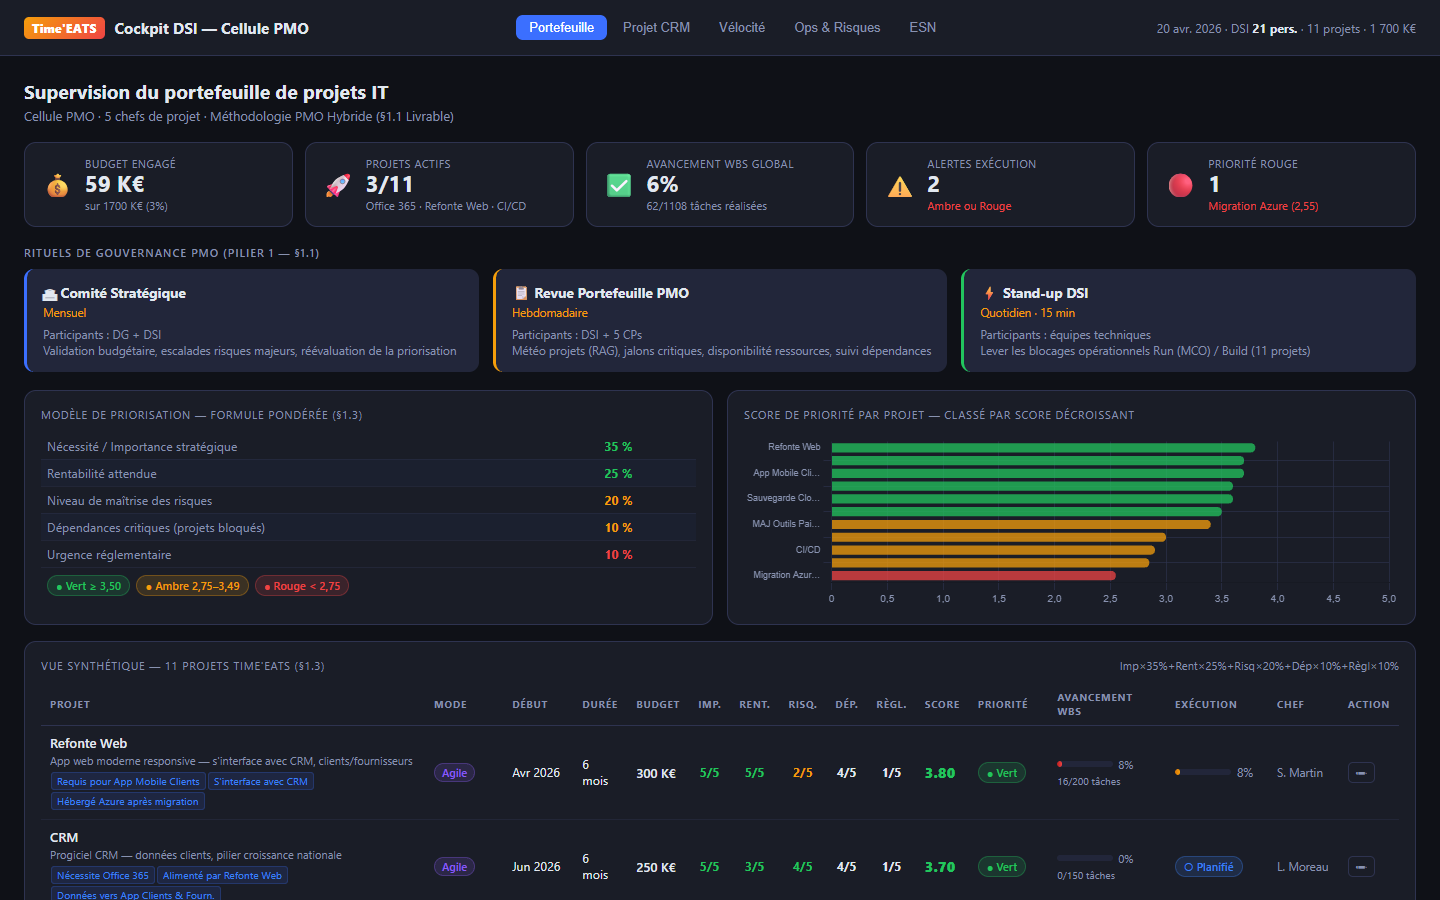
\includegraphics[width=\textwidth,keepaspectratio]{cockpit_portefeuille.png}
  \par\vspace{4pt}
  {\small\textcolor{cnSlate}{\textit{Capture --- Onglet Portefeuille : supervision des 11 projets, score de priorisation, RAG exécution.}}}
\end{center}

\vspace{6pt}
\begin{center}
  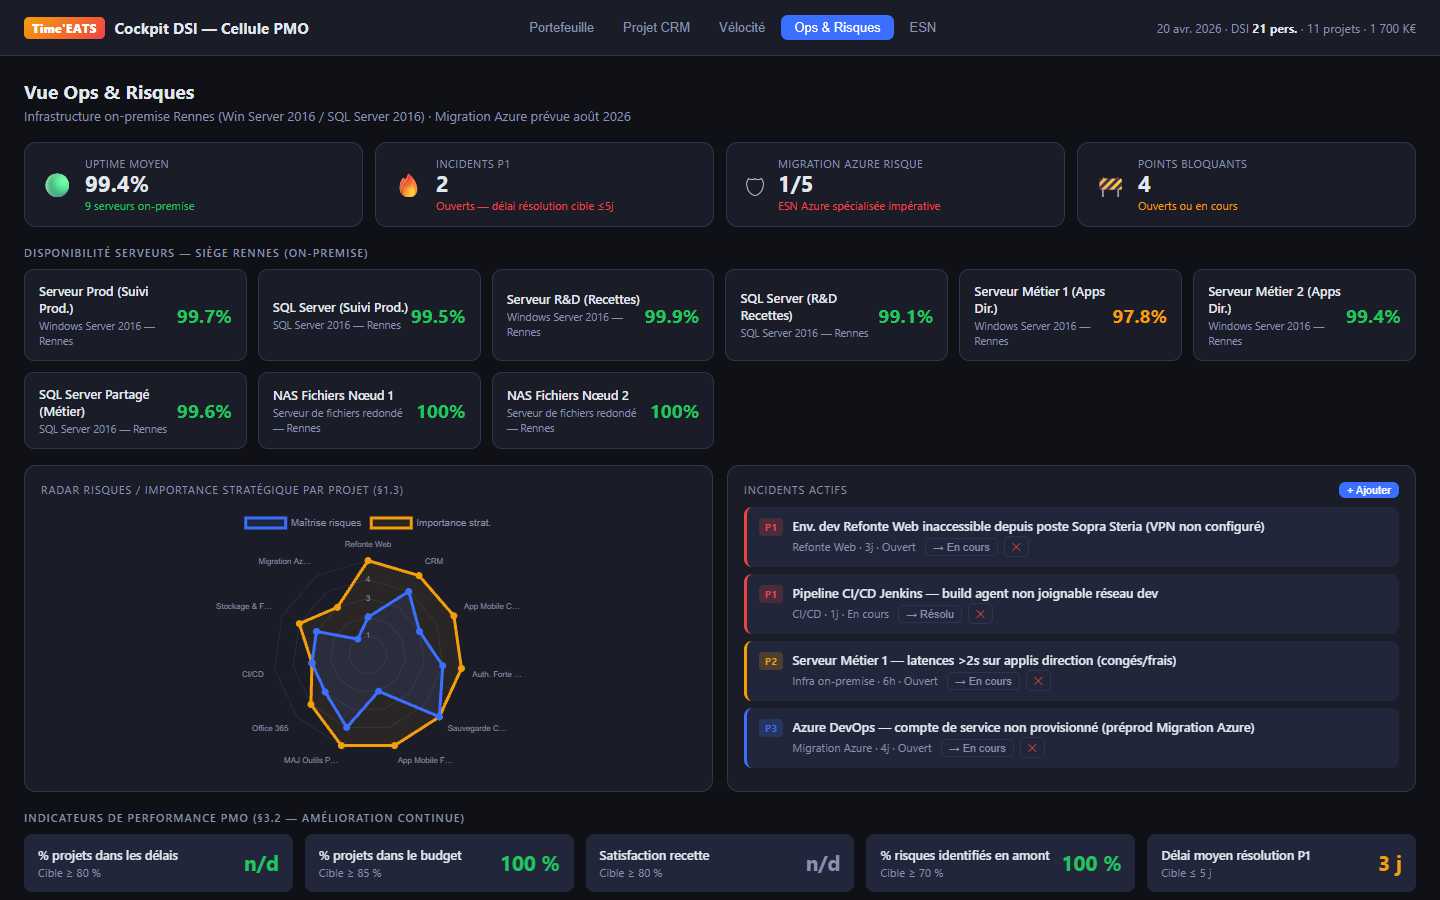
\includegraphics[width=\textwidth,keepaspectratio]{cockpit_ops.png}
  \par\vspace{4pt}
  {\small\textcolor{cnSlate}{\textit{Capture --- Onglet Ops \& Risques : uptime serveurs, incidents P1/P2/P3, KPIs PMO.}}}
\end{center}

\section{Capitalisation et amélioration continue}

La DSI pilote 11 projets avec 5 chefs de projet. Sans capitalisation structurée, chaque erreur sera répétée et chaque bonne pratique perdue. L'amélioration continue est un \textbf{levier de productivité immédiat} --- et sa mise en œuvre ne requiert aucun budget supplémentaire.

\subsection*{Processus de capitalisation --- 4 étapes}

\begin{center}
\renewcommand{\arraystretch}{1.5}
\begin{tabularx}{\textwidth}{C{1cm} L{3.8cm} L{5.5cm} L{3.5cm}}
\toprule
\rowcolor{cnNavy}
\th{Étape} & \th{Activité} & \th{Description} & \th{Outil} \\
\midrule
1 & Rétrospective de clôture & Séance 2h avec l'équipe : ce qui a fonctionné, ce qui a posé problème, 3 actions d'amélioration & Teams / Miro \\
\rowcolor{cnIce}
2 & Rédaction fiche REX (P5-23) & Synthèse structurée : contexte, enseignements, recommandations, fichiers liés & SharePoint O365 \\
3 & Mise à jour du référentiel & Templates concernés mis à jour, bonnes pratiques PMO enrichies & SharePoint O365 \\
\rowcolor{cnIce}
4 & Revue semestrielle PMO & Analyse des REX accumulés, patterns récurrents, mise à jour du référentiel & COPIL semestriel \\
\bottomrule
\end{tabularx}
\end{center}

\subsection*{Boucle PDCA appliquée au PMO}

\begin{itemize}
  \item \textbf{Plan} : Définir les processus PMO et les templates du référentiel (Ch.\ 3 du présent livrable).
  \item \textbf{Do} : Appliquer le référentiel sur chaque projet du portefeuille (Partie II : exemple Refonte Web).
  \item \textbf{Check} : Collecter les REX à la clôture ; mesurer les indicateurs PMO (respect budgétaire, taux de jalons, satisfaction métier).
  \item \textbf{Act} : Mettre à jour le référentiel sur la base des enseignements ; présenter au COPIL semestriel.
\end{itemize}

\begin{reco}
Cette démarche ne représente \textbf{aucun coût additionnel} : le Cockpit DSI s'appuie sur Node.js (runtime gratuit) et SharePoint Online (déjà financé par le projet Office 365). La satisfaction client et le bien-être équipe remontent naturellement du niveau projet vers le PMO --- sans double saisie.
\end{reco}

\newpage

% ============================================================
% PARTIE II — APPLICATION AU PROJET REFONTE WEB
% ============================================================
\part{Application au projet Refonte Web}

% ============================================================
% CHAPITRE 5 — CADRAGE DU PROJET REFONTE WEB
% ============================================================
\chapter{Cadrage du projet Refonte Web}

\begin{finding}
La \textbf{Refonte Web} est le projet le mieux noté du portefeuille (score 3{,}80/5 --- RAG Vert). Elle constitue la \textbf{pierre angulaire de l'écosystème digital cible} : socle commun à toute la transformation (CRM, App Clients, App Fournisseurs) via une API publique, et levier de conversion direct pour Marketing et Commerce. Démarrage 22/04/2026 --- Go-Live impératif 30/09/2026 --- Budget ferme 300~K€.
\end{finding}

\section{Carte d'identité du projet}

\renewcommand{\arraystretch}{1.5}
\begin{tabularx}{\textwidth}{L{4cm} Y L{4cm} Y}
\toprule
\rowcolor{cnNavy}\th{Champ} & \th{Valeur} & \th{Champ} & \th{Valeur} \\
\midrule
Code projet      & REF-WEB-2026                & Statut au 19/05  & \ragV --- 8\,\% avancement \\
\rowcolor{cnIce}
Chef de projet   & M. X                        & Sponsor          & Mme Y (DSI) \\
Date de démarrage & 22/04/2026                 & Date de Go-Live  & 30/09/2026 \\
\rowcolor{cnIce}
Budget total     & 300~K€ (ferme)              & Mode             & Hybride (Waterfall + Scrum) \\
ESN partenaire   & Sopra Steria (forfait 400 j/h --- 200~K€) & PMO référent     & M. L \\
\rowcolor{cnIce}
Hébergement      & Azure West Europe (Paris)   & Conformité       & RGAA 4.1 AA + RGPD + OWASP ASVS 2 \\
\bottomrule
\end{tabularx}

\section{Enjeux et objectifs SMART}

\renewcommand{\arraystretch}{1.4}
\begin{tabularx}{\textwidth}{C{1cm} L{5cm} L{3cm} C{2.5cm} L{3cm}}
\toprule
\rowcolor{cnNavy}\th{\#} & \th{Objectif} & \th{Mesure} & \th{Cible} & \th{Échéance} \\
\midrule
O1 & Trafic organique national & Sessions GA4 & +30\,\% vs T1 2026 & M+6 post Go-Live \\
\rowcolor{cnIce}
O2 & Taux de conversion        & Funnel commande & 1{,}0\,\% $\rightarrow$ 2{,}2\,\% & M+9 \\
O3 & Performance Web Vitals    & Lighthouse Perf./A11y & $\geq$ 90 sur 10 parcours & J5 (Go-Live) \\
\rowcolor{cnIce}
O4 & Délai de publication CMS  & Mesure CMS (création $\rightarrow$ publication) & $<$ 30 min (vs 5 j) & J5+30 \\
O5 & API REST v1 documentée    & OpenAPI 3.0 + couverture tests & 100\,\% endpoints publics & J2 (30/06) \\
\rowcolor{cnIce}
O6 & TCO à 12 mois             & Hébergement + licences + run & $-25\,\%$ vs Drupal legacy & M+12 \\
\bottomrule
\end{tabularx}

\section{Périmètre et options}

\renewcommand{\arraystretch}{1.3}
\begin{tabularx}{\textwidth}{L{1.5cm} Y}
\toprule
\rowcolor{cnNavy}\th{} & \th{Description} \\
\midrule
\cellcolor{cnGreen!20}\textbf{In} & Site corporate (10 templates UX/UI), CMS contributeur autonome, espace client (compte, commandes, factures), API publique REST v1, SEO technique, conformité RGAA 4.1 AA / RGPD, SSO Office 365 (ou IdP local en repli), CI/CD multi-env, monitoring APM. \\
\rowcolor{cnIce}
\cellcolor{cnRed!20}\textbf{Out} & Refonte CRM (projet dédié), applications mobiles, tunnel B2B avancé, back-office logistique, migration contenus legacy antérieurs 2024, refonte intranet collaborateur. \\
\bottomrule
\end{tabularx}

\vspace{4pt}
\begin{decision}
Trois options étudiées (cf.\ \texttt{projets/refonte\_web/P1-02\_note\_de\_cadrage.tex}, §7) : \textbf{Option A retenue} (refonte complète Next.js + Headless CMS + API), Option B (upgrade Drupal incrémental --- écartée car n'adresse pas l'industrialisation), Option C (SaaS Shopify/Salesforce --- écartée pour verrouillage éditeur).
\end{decision}

\section{Approche hybride retenue}

\begin{itemize}
  \item \textbf{Phases 1, 2 et 5 (Démarrage, Planification, Clôture) en Waterfall} : baselines contractuelles (charte, PMP, WBS, Gantt, budget, risques), recette PV, transfert exploitation.
  \item \textbf{Phases 3 et 4 (Exécution, Maîtrise) en Scrum 2 semaines} : 8 sprints prévus (S22 à S37), démos COPIL aux jalons J1--J4, vélocité tracée dans Azure DevOps Boards.
  \item \textbf{Gouvernance} : COPIL mensuel (3\textsuperscript{e} mardi), daily Scrum quotidien, revue/rétrospective bi-mensuelle, rapport d'avancement à l'\textbf{ouverture} de chaque mois.
\end{itemize}

\newpage

% ============================================================
% CHAPITRE 6 — PILOTAGE OPÉRATIONNEL
% ============================================================
\chapter{Pilotage opérationnel du projet Refonte Web}

\section{Jalons baseline}

\renewcommand{\arraystretch}{1.4}
\begin{tabularx}{\textwidth}{C{1cm} L{5cm} C{2.5cm} Y}
\toprule
\rowcolor{cnNavy}\th{N°} & \th{Jalon} & \th{Date baseline} & \th{Condition de franchissement} \\
\midrule
J0 & Kick-off projet            & 22/04/2026 & Charte signée + équipe staffée \\
\rowcolor{cnIce}
J1 & Maquettes UX validées      & 27/05/2026 & Design system v1 + parcours-clés signés MOA \\
J2 & Socle technique validé     & 30/06/2026 & API v1 testée + CI/CD opérationnelle + envs prêts \\
\rowcolor{cnIce}
J3 & MVP fonctionnel staging    & 31/07/2026 & Site + CMS + espace client en démo MOA \\
J4 & Recette + audits OK        & 31/08/2026 & PV recette signé + RGAA AA + OWASP ASVS 2 \\
\rowcolor{cnIce}
J5 & Go-Live production         & 30/09/2026 & Bascule réussie + monitoring run + REX \\
\bottomrule
\end{tabularx}

\section{WBS --- vue tabulaire synthétique}

\renewcommand{\arraystretch}{1.3}
\begin{tabularx}{\textwidth}{C{1cm} L{5.5cm} C{2cm} Y}
\toprule
\rowcolor{cnNavy}\th{Lot} & \th{Libellé} & \th{Charge (j.h)} & \th{Responsable} \\
\midrule
1 & Démarrage                    & 14  & CP (M. X) \\
\rowcolor{cnIce}
2 & Planification                & 28  & CP + PMO \\
3 & UX/UI \& Design System       & 63  & UX (Mme C) + ESN \\
\rowcolor{cnIce}
4 & Socle technique \& API       & 88  & Tech Lead (M. A) + ESN \\
5 & Réalisation produit          & 202 & ESN Sopra Steria + équipe interne \\
\rowcolor{cnIce}
6 & Qualité \& Recette           & 65  & RSSI + ESN + audits externes \\
7 & Conduite du changement       & 20  & CP + Marketing \\
\rowcolor{cnIce}
8 & Clôture \& Go-Live           & 22  & CP + DSI Ops \\
\midrule
\rowcolor{cnNavy!10}\textbf{TOTAL} & & \textbf{\textasciitilde 480 j.h} & (incl.\ ESN 400 j.h forfait) \\
\bottomrule
\end{tabularx}

\vspace{4pt}
\textit{Détail complet par work package : cf.\ \texttt{projets/refonte\_web/pdf/P2-06\_wbs.pdf}.}

\section{WBS --- vue graphique}

\begin{center}
  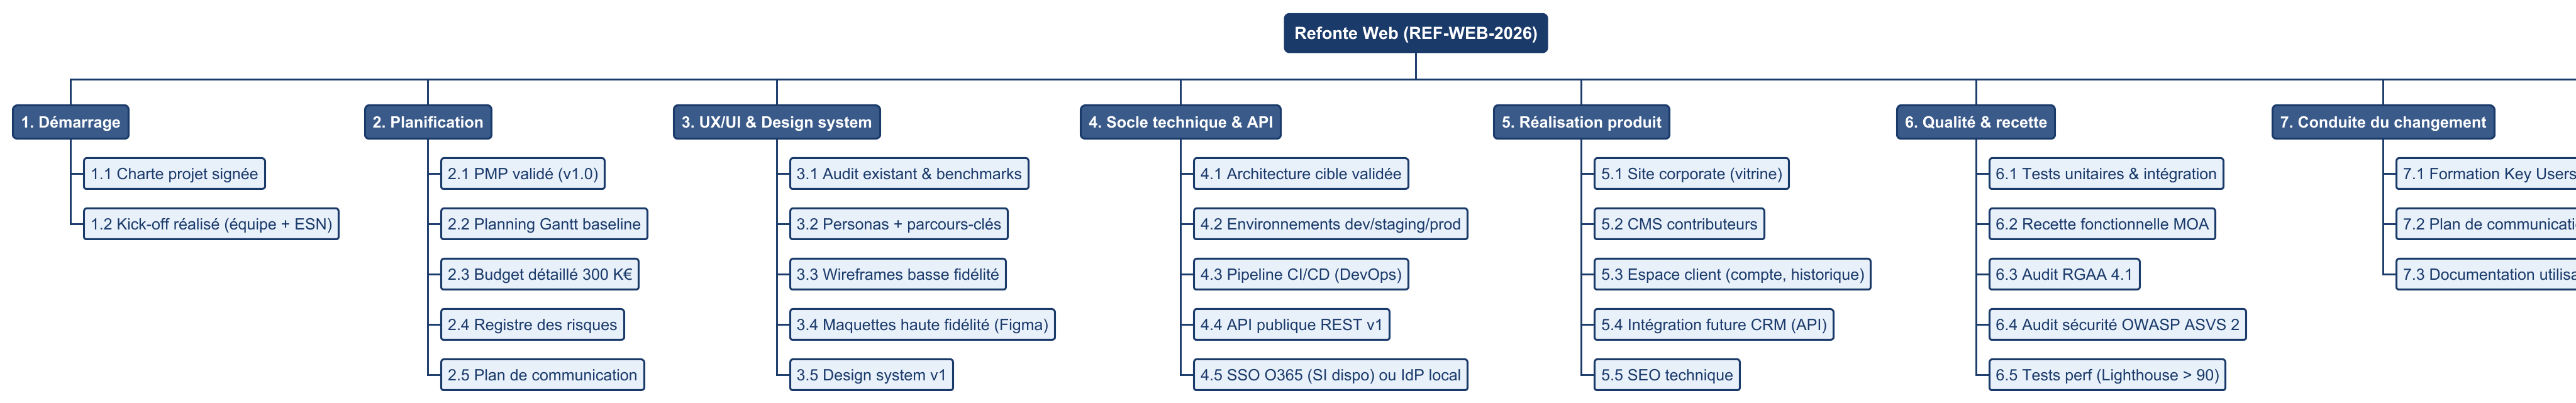
\includegraphics[width=\textwidth,keepaspectratio]{wbs_refonte_web.png}
  \par\vspace{4pt}
  {\small\textcolor{cnSlate}{\textit{WBS Refonte Web --- arborescence à 3 niveaux : projet $\rightarrow$ 8 lots $\rightarrow$ 34 work packages.}}}
\end{center}

\newpage

\section{Budget --- synthèse}

\renewcommand{\arraystretch}{1.4}
\begin{tabularx}{\textwidth}{L{5cm} C{2cm} C{2cm} Y}
\toprule
\rowcolor{cnNavy}\th{Poste} & \th{Type} & \th{Montant} & \th{Commentaire} \\
\midrule
Intégration ESN Sopra Steria & CAPEX & 200~K€ & Forfait 400 j/h \\
\rowcolor{cnIce}
Ressources internes valorisées & Interne & 80~K€  & 4{,}5 ETP cumulés sur 6 mois \\
Licences \& SaaS (CMS, Figma, APM) & OPEX & 7~K€   & Sur la durée du projet \\
\rowcolor{cnIce}
Hébergement Azure West Europe & CAPEX & 6~K€   & 3 environnements 6 mois \\
Audits externes (RGAA + OWASP) & OPEX & 4~K€   & 1 audit + 1 pentest \\
\rowcolor{cnIce}
Réserve pour aléas             & Réserve & 3~K€   & Sur arbitrage COPIL \\
\midrule
\rowcolor{cnNavy!10}\textbf{TOTAL} & & \textbf{300~K€} & Ventilation détaillée P2-08 \\
\bottomrule
\end{tabularx}

\textit{Détail mensuel + suivi EVM : cf.\ \texttt{projets/refonte\_web/pdf/P2-08\_budget\_previsionnel.pdf}.}

\section{Risques majeurs (top 7)}

\renewcommand{\arraystretch}{1.3}
\begin{tabularx}{\textwidth}{C{0.7cm} L{5cm} C{1cm} C{1cm} C{1.5cm} L{4.5cm}}
\toprule
\rowcolor{cnNavy}\th{\#} & \th{Risque} & \th{P} & \th{I} & \th{Score} & \th{Mitigation} \\
\midrule
R1 & Retard Office 365 / SSO            & 3 & 4 & \cellcolor{cnOrange!20}\textbf{12} & Repli IdP local prévu (8~K€ provisionnés) \\
\rowcolor{cnIce}
R2 & Non-conformité RGAA 4.1 AA         & 3 & 4 & \cellcolor{cnOrange!20}\textbf{12} & Pré-audit S30 + revue UX experte \\
R3 & Sous-effectif ESN sprint critique  & 3 & 3 & \cellcolor{cnOrange!20}\textbf{9}  & Clause continuité + backup nominatif \\
\rowcolor{cnIce}
R4 & Indispo. référent Marketing        & 2 & 4 & \cellcolor{cnOrange!20}\textbf{8}  & Suppléant désigné + créneaux sanctuarisés \\
R5 & Migration Azure non finalisée à J2 & 2 & 4 & \cellcolor{cnOrange!20}\textbf{8}  & Coord. weekly Infra + tenant repli \\
\rowcolor{cnIce}
R6 & Web Vitals dégradés                & 3 & 3 & \cellcolor{cnOrange!20}\textbf{9}  & Lighthouse en CI + budget JS $<$ 200 ko \\
R7 & Vulnérabilité OWASP critique       & 2 & 5 & \cellcolor{cnRed!20}\textbf{10}    & SAST/CodeQL + threat modeling + code review RSSI \\
\bottomrule
\end{tabularx}

\textit{Registre complet : cf.\ \texttt{projets/refonte\_web/pdf/P2-09\_registre\_risques.pdf}.}

\section{Tableau de bord projet (cockpit) --- état au 19/05/2026}

\renewcommand{\arraystretch}{1.4}
\begin{tabularx}{\textwidth}{L{4cm} C{2cm} C{2cm} C{2cm} Y}
\toprule
\rowcolor{cnNavy}\th{Indicateur} & \th{Valeur} & \th{Seuil} & \th{Statut} & \th{Commentaire} \\
\midrule
Avancement physique     & 8\,\%     & Selon phase & \ragV & Conforme phase Planification \\
\rowcolor{cnIce}
Budget consommé         & 35~K€ (11{,}7\,\%) & $\leq$ \% av.\ +5pt & \ragA & Légère avance consommation \\
IPC                     & 0{,}98    & $\geq$ 0{,}95   & \ragV & Aligné valeur acquise \\
\rowcolor{cnIce}
IPD                     & 0{,}93    & $\geq$ 0{,}95   & \ragA & PMP livré J+2 \\
Jalons respectés        & 100\,\%   & $\geq$ 80\,\%   & \ragV & J0 OK, J1 en trajectoire \\
\rowcolor{cnIce}
Risques critiques actifs & 0        & 0               & \ragV & 7 risques Élevés, 0 Critique \\
Anomalies bloquantes    & 0         & 0               & \ragV & Aucune ouverte \\
\bottomrule
\end{tabularx}

\textit{Rapport d'avancement détaillé : cf.\ \texttt{projets/refonte\_web/pdf/P3-13\_rapport\_avancement.pdf}.}

\newpage

% ============================================================
% CHAPITRE 7 — DOSSIER PMP REFONTE WEB (RENVOI)
% ============================================================
\chapter{Dossier PMP Refonte Web --- documents instanciés}

\begin{finding}
Le pilotage opérationnel de la Refonte Web s'appuie sur un \textbf{dossier compagnon} (\texttt{pmp\_refonte\_web.pdf}) qui rassemble les \textbf{15 documents instanciés} à partir des templates du référentiel (Ch.\ 3). Chaque document est compilé en PDF autonome dans \texttt{projets/refonte\_web/pdf/}. Le présent chapitre fait office d'\textbf{index navigationnel}.
\end{finding}

\section{Architecture du dossier compagnon}

\begin{itemize}
  \item \textbf{Document maître} : \texttt{pmp\_refonte\_web.pdf} --- index, carte d'identité, table des documents instanciés, engagements contractuels.
  \item \textbf{Document pivot} : \texttt{P2-05\_plan\_management\_projet.pdf} --- Plan de Management Projet en 11 sections (PMBOK 7\textsuperscript{e} + PRINCE2 + ADKAR).
  \item \textbf{14 documents annexes} --- charte, note de cadrage, PBS, CDC, fiche d'identification, RACI, WBS, Gantt, budget, risques, communication, conduite du changement, CR de réunion (kick-off), rapport d'avancement (M+1).
\end{itemize}

\section{Index des 15 documents instanciés}

\noindent\textit{Tous les chemins sont préfixés par \texttt{projets/refonte\_web/pdf/} et le fichier source équivalent se trouve dans \texttt{projets/refonte\_web/}.}

\vspace{4pt}

\renewcommand{\arraystretch}{1.3}
\newcommand{\pthi}[1]{{\tiny\ttfamily #1}}
\begin{longtable}{C{1.1cm} L{5cm} C{2cm} L{5.5cm} C{1cm}}
\toprule
\rowcolor{cnNavy}
\th{ID} & \th{Document} & \th{Phase} & \th{Fichier PDF instancié} & \th{Statut} \\
\midrule
\endhead
\bottomrule
\endfoot

\multicolumn{5}{l}{\cellcolor{cnNavy!15}\textbf{\textcolor{cnNavy}{Phase 1 --- Démarrage}}} \\
\midrule
P1-01 & Charte projet                  & Démarrage     & \pthi{P1-01\_charte\_projet.pdf}         & \ragV \\
\rowcolor{cnIce}
P1-02 & Note de cadrage                & Démarrage     & \pthi{P1-02\_note\_de\_cadrage.pdf}      & \ragV \\
P1-02bis & Product Breakdown Structure (PBS) & Démarrage & \pthi{P1-02bis\_pbs.pdf}              & \ragV \\
\rowcolor{cnIce}
P1-02ter & Cahier des charges (CDC)    & Démarrage     & \pthi{P1-02ter\_cdc.pdf}                 & \ragV \\
P1-03 & Fiche d'identification         & Démarrage     & \pthi{P1-03\_fiche\_identification.pdf}  & \ragV \\
\rowcolor{cnIce}
P1-04 & Matrice RACI                   & Démarrage     & \pthi{P1-04\_matrice\_raci.pdf}          & \ragV \\
\midrule

\multicolumn{5}{l}{\cellcolor{cnNavy!15}\textbf{\textcolor{cnNavy}{Phase 2 --- Planification}}} \\
\midrule
P2-05 & \textbf{Plan de Management Projet} (pivot) & Planification & \pthi{P2-05\_plan\_management\_projet.pdf} & \ragV \\
\rowcolor{cnIce}
P2-06 & WBS (tabulaire + graphique PNG) & Planification & \pthi{P2-06\_wbs.pdf}                  & \ragV \\
P2-07 & Planning Gantt baseline        & Planification & \pthi{P2-07\_planning\_gantt.pdf}        & \ragV \\
\rowcolor{cnIce}
P2-08 & Budget prévisionnel + EVM      & Planification & \pthi{P2-08\_budget\_previsionnel.pdf}   & \ragV \\
P2-09 & Registre des risques v1        & Planification & \pthi{P2-09\_registre\_risques.pdf}      & \ragV \\
\rowcolor{cnIce}
P2-10 & Plan de communication          & Planification & \pthi{P2-10\_plan\_communication.pdf}    & \ragV \\
P2-11 & Plan de conduite du changement & Planification & \pthi{P2-11\_plan\_conduite\_changement.pdf} & \ragV \\
\midrule

\multicolumn{5}{l}{\cellcolor{cnNavy!15}\textbf{\textcolor{cnNavy}{Phase 3 --- Exécution (exemples)}}} \\
\midrule
\rowcolor{cnIce}
P3-12 & CR Kick-off (22/04/2026)       & Exécution     & \pthi{P3-12\_cr\_reunion.pdf}            & \ragV \\
P3-13 & Rapport d'avancement (mai 2026)& Exécution     & \pthi{P3-13\_rapport\_avancement.pdf}    & \ragV \\
\end{longtable}

\section{Documents à produire au fil de l'avancement}

\begin{finding}
Au-delà des 15 documents déjà instanciés, le pilotage Phase 3--5 génère les livrables suivants à produire au fil de l'eau à partir des templates du référentiel.
\end{finding}

\renewcommand{\arraystretch}{1.3}
\begin{tabularx}{\textwidth}{C{1.2cm} L{5cm} C{2.5cm} Y}
\toprule
\rowcolor{cnNavy}\th{ID} & \th{Document} & \th{Fréquence} & \th{Première occurrence prévue} \\
\midrule
P3-12 (suite) & CR de réunion sprint / COPIL & Tous les 15 j / Mensuel & Sprint 1 Review --- 13/06/2026 \\
\rowcolor{cnIce}
P3-13 (suite) & Rapport d'avancement mensuel & Mensuel             & Juin 2026 (diffusé 05/07) \\
P3-14         & Demande de changement        & Sur événement       & À anticiper en juillet \\
\rowcolor{cnIce}
P3-15         & Log des anomalies            & Vivant              & Dès la recette (août 2026) \\
P4-16         & Tableau de bord projet       & Mensuel             & Mai 2026 (intégré cockpit) \\
\rowcolor{cnIce}
P4-17         & Rapport d'écarts             & Sur seuil dépassé   & Si IPC ou IPD $<$ 0{,}90 \\
P4-18         & CR / Slides COPIL            & Mensuel             & COPIL inception 20/05/2026 \\
\rowcolor{cnIce}
P5-19         & PV de recette fonctionnelle  & 1 fois              & 31/08/2026 (J4) \\
P5-20         & PV de recette technique      & 1 fois              & 31/08/2026 (J4) \\
\rowcolor{cnIce}
P5-21         & Rapport de clôture           & 1 fois              & 30/09/2026 (J5) \\
P5-22         & PV transfert exploitation    & 1 fois              & 30/09/2026 (J5) \\
\rowcolor{cnIce}
P5-23         & Fiche REX                    & 1 fois              & 15/10/2026 (J5+15) \\
P5-24         & Lettre de fin de mission ESN & 1 fois              & 30/09/2026 (solde Sopra Steria) \\
\bottomrule
\end{tabularx}

\begin{reco}
À chaque nouvelle occurrence d'un document Phase 3--5, le CP :
\begin{enumerate}
  \item Duplique le template depuis \texttt{referentiel/} vers \texttt{projets/refonte\_web/}.
  \item Renseigne les champs spécifiques au projet et compile en PDF dans \texttt{projets/refonte\_web/pdf/}.
  \item Met à jour la table de la section 2 du dossier compagnon \texttt{pmp\_refonte\_web.pdf}.
  \item Versionne dans SharePoint et notifie le PMO pour intégration au cockpit DSI.
\end{enumerate}
\end{reco}

\begin{alert}
\textbf{Document maître} : en cas de divergence entre ce livrable principal et le dossier compagnon \texttt{pmp\_refonte\_web.pdf}, c'est le \textbf{dossier compagnon} qui fait \textbf{foi pour le projet Refonte Web} (granularité plus fine, données à jour). Le présent livrable sert de référence \textbf{méthodologique} pour l'ensemble du portefeuille.
\end{alert}

\vfill
\begin{center}
\tiny\textcolor{cnSlate}{Document confidentiel --- Cellule PMO --- Time'Eats --- CESI MAALSI 2026}
\end{center}

\end{document}
